\chapter{Modelization of central perpspective cameras}


%-----------------------------------------------------
%-----------------------------------------------------
%-----------------------------------------------------

\section{Introduction}

In this chapter we introduce the mathematical model used in {\tt MMVII}
for modelization of central perspective camera.  The majority (if not all)
of images we manipulate in current life are acquired by central perspective camera, it includes
smarthphone cameras,  reflex cameras,  most aerial cameras \dots  In fact they are so common that
it is easier to define camera that are not central  perspective :
it include majority of satellite images and few aerial camera (like leica-ADS40).

We start from the most basic model and introduce progressively different refinement,
being cautious to justify by physic considerations all the parametric terms we introduce.
We also introduce the convention selected in {\tt MMVII} as in photogrammetry/computer vision
there are several arbitrary choices that may be confusing.

%-----------------------------------------------------
%-----------------------------------------------------
%-----------------------------------------------------

\section{Camera Obscura and  central perspective model}

%-----------------------------------------------------
\subsection{Physicall model}

\begin{figure}
\centering
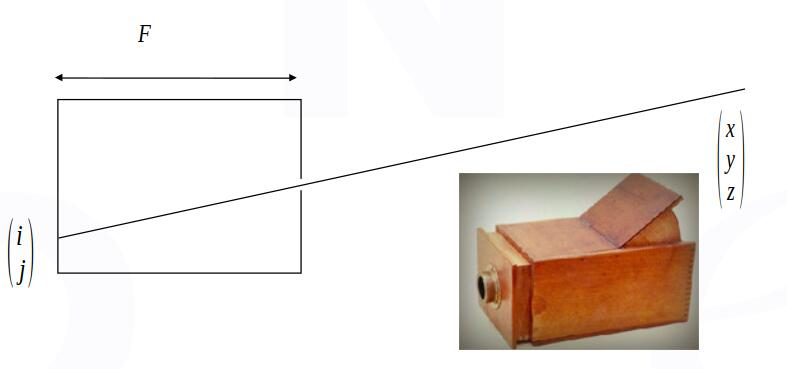
\includegraphics[width=12cm]{Methods/Images/CameraObscura.jpg}\caption{Camera osbcura : schema and a real object}
	\label{fig:CameraObscura}
\end{figure}


We begin by the description of very simple object, but which is really a the origin of
the photography and, in some way, is the simplest possible camera  :  the camera obscura.
Basically it can be described as a box with a hole, at the entrance of the box we have
a the hole that let the light in, and at the bottom of the box we have the film of
the camera. 

Figure~\ref{fig:CameraObscura} presents a real camera and a basic schema showing
the construction of the image :  to compute the image of a point $P^c=x^c,y^c,z^c$ of the real scene
we juts have to trace the line starting from $P^c$, going throw the hole and take its intersection $q=i,j$
with the image plane.


%-----------------------------------------------------
\subsection{Setting equations}

To compute a mathematical relation between $x^c,y^c,z^c$ and $i,j$ we will introduce several hypothesis 
and notations illustrated by figure~\ref{fig:Camera3DNote} :

\begin{figure}
\centering
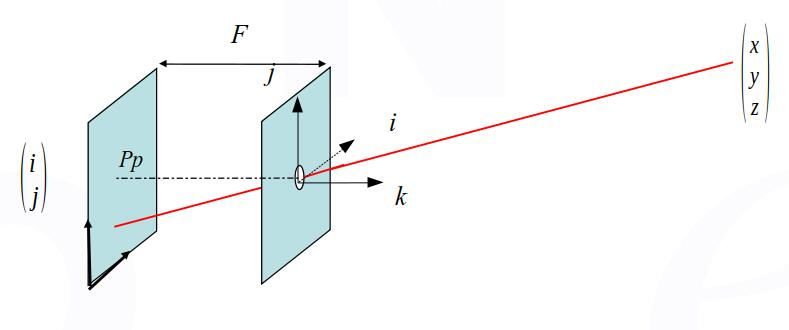
\includegraphics[width=12cm]{Methods/Images/Camera3D.jpg}\caption{Notation for camera relation}
	\label{fig:Camera3DNote}
\end{figure}

\begin{itemize}
	\item for 3d coordinates, we consider a local $3d$ repair $(O,\vec{i},\vec{j},\vec{k})$  where $O$ is the entrance hole,
              $\vec{i},\vec{j}$ belongs to the image plane and $\vec{k}$ is orthogonal to  $\vec{i}$ and $\vec{j}$;

	\item for $i,j$ we consider a image repair originated at one corner $c$ of the box;

	\item we note $P^p$ (principal point)  the intersection of axe $O\vec{k}$  with the image plane,
	      and $F$ (focal length) the distance between $P^p$ and $O$.

        \item we note $Q_3$  the $3d$ point corresponding to $q$.

\end{itemize}

To compute coordinates of $Q_3$ we can use chasles relation as indicated in equation~\ref{PC:Chasles} :

\begin{equation}
	\overrightarrow{OQ_3} =  \overrightarrow{O P^p} + \overrightarrow{P^p c} +  \overrightarrow{c Q_3}
	 =     \begin{pmatrix} 0\\0\\-F \end{pmatrix}
             + \begin{pmatrix} -P^p_x\\-P^p_y\\0 \end{pmatrix}
             + \begin{pmatrix} i\\j\\0 \end{pmatrix}
	 =     \begin{pmatrix} i-P^p_x\\j-P^p_y\\-F \end{pmatrix}
	\label{PC:Chasles}
\end{equation}

Now remind that light having a straight path, the $3$ point $Q_3$, $0$ and $P^c$ must be aligned,
which can be wrotten by equation~\ref{PC:Alignment} :

\begin{equation}
	\exists \lambda : 
	\begin{pmatrix} i-P^p_x\\j-P^p_y\\-F \end{pmatrix} 
      = \lambda   \begin{pmatrix} x^c\\y^c\\z^c \end{pmatrix}
		\label{PC:Alignment}
\end{equation}

By a simple quotient  we can elimimnate $\lambda$ in~\ref{PC:Alignment} and obtain :


\begin{equation}
	i = P^p_x -F \frac{x^c}{z^c}  \; ; \;
	j = P^p_y -F \frac{y^c}{z^c}  
	\label{PC:FormulaImaIntr1}
\end{equation}

%-----------------------------------------------------
\subsection{Local image formula}

The usage is to modiy the equation~\ref{PC:FormulaImaIntr1} by changing the sign of $F$;
this comes to consider a camera model ,
 not physically feasible and slightly different from the camera obscura,  
where the image plane is before the whole instead of behind, and that
is illustrated by figure~\ref{fig:PcInvCam}.  

\begin{figure}
\centering
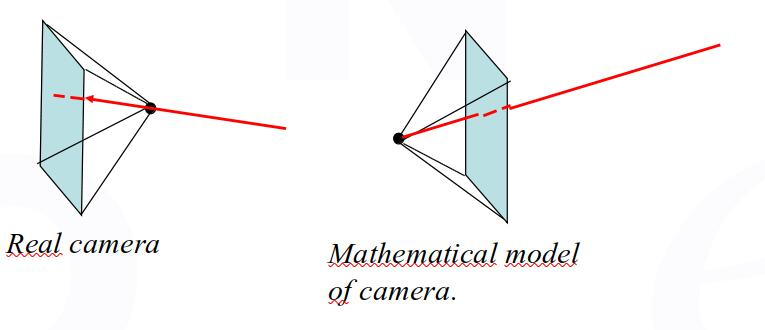
\includegraphics[width=12cm]{Methods/Images/InvCamera.jpg}
	\caption{Camera model : physically based one (left) and used one (right)}
	\label{fig:PcInvCam}
\end{figure}

Finally we will use equation~\ref{PC:FormulaImaIntr2} to formulate the relation between
local ground coordinates $P^c$  and image coordinate for this basic camera :

\begin{equation}
	i = P^p_x +F \frac{x^c}{z^c}  \; ; \;
	j = P^p_y +F \frac{y^c}{z^c}  
	\label{PC:FormulaImaIntr2}
\end{equation}

Setting the canonical projection $\pi_0$:

\begin{equation}
	  \pi_0 \begin{pmatrix} x^c \\ y^c \\ z^c \end{pmatrix} 
           =  \begin{pmatrix} \frac{x^c}{z^c} \\  \frac{x^c}{z^c}  \end{pmatrix} 
\end{equation}

and the intrinsic calibration $ \mathcal{I}_0$ :

\begin{equation}
	   \mathcal{I}_0  \begin{pmatrix} u \\  v  \end{pmatrix} 
		   =  P^p + F  \begin{pmatrix} u \\  v  \end{pmatrix}  \label{EqIntNoDist}
\end{equation}

we will write :

\begin{equation}
	q  =   \mathcal{I}_0 (\pi_0 (P^c))
\end{equation}


%-----------------------------------------------------
\subsection{Global image formula}

Generally we need to write the coordinate of $q$ as a function of the global coordinate $P$ or a point.
For this we just have to write the local coordinates $P^c$ as a function of global $P$, 
we use $C$ the center of the camera, and $R$ its orientation :

\begin{equation}
	P =  C+ R *P_c
\end{equation}

Which give the image formula :
\begin{equation}
	q  =   \mathcal{I}_0 (\pi_0 (^t R (P - C))) \label{FormImage0}
\end{equation}

This formula will follow us for a long time. The main thing that will evolve is $\mathcal{I}_0$,
and later $\pi_0$,
that will become more sophisticated to take into account lenses used in real camera.


%-----------------------------------------------------
\subsection{A remark on repair orientation}

We have not discussed untill now which image repair is used for image coordnates $i,j$.
The choice done in {\tt MMVII} is to use the coordinate system of majority of images
processing solution; that is : $i$ is left to right and $j$ is up to bottom.

As we aline  local repair $(O,\vec{i},\vec{j},\vec{k})$  on this coordinate system ,
and we want a direct $3d$ repair with $\vec{k} = \vec{i} \wedge \vec{j} $, this
has for consequences that the axe $O\vec{k})$ is in the viewewing direction of the
camera.  The figure~\ref{fig:FormIm} illustrates this convention;


\begin{figure}
\centering
	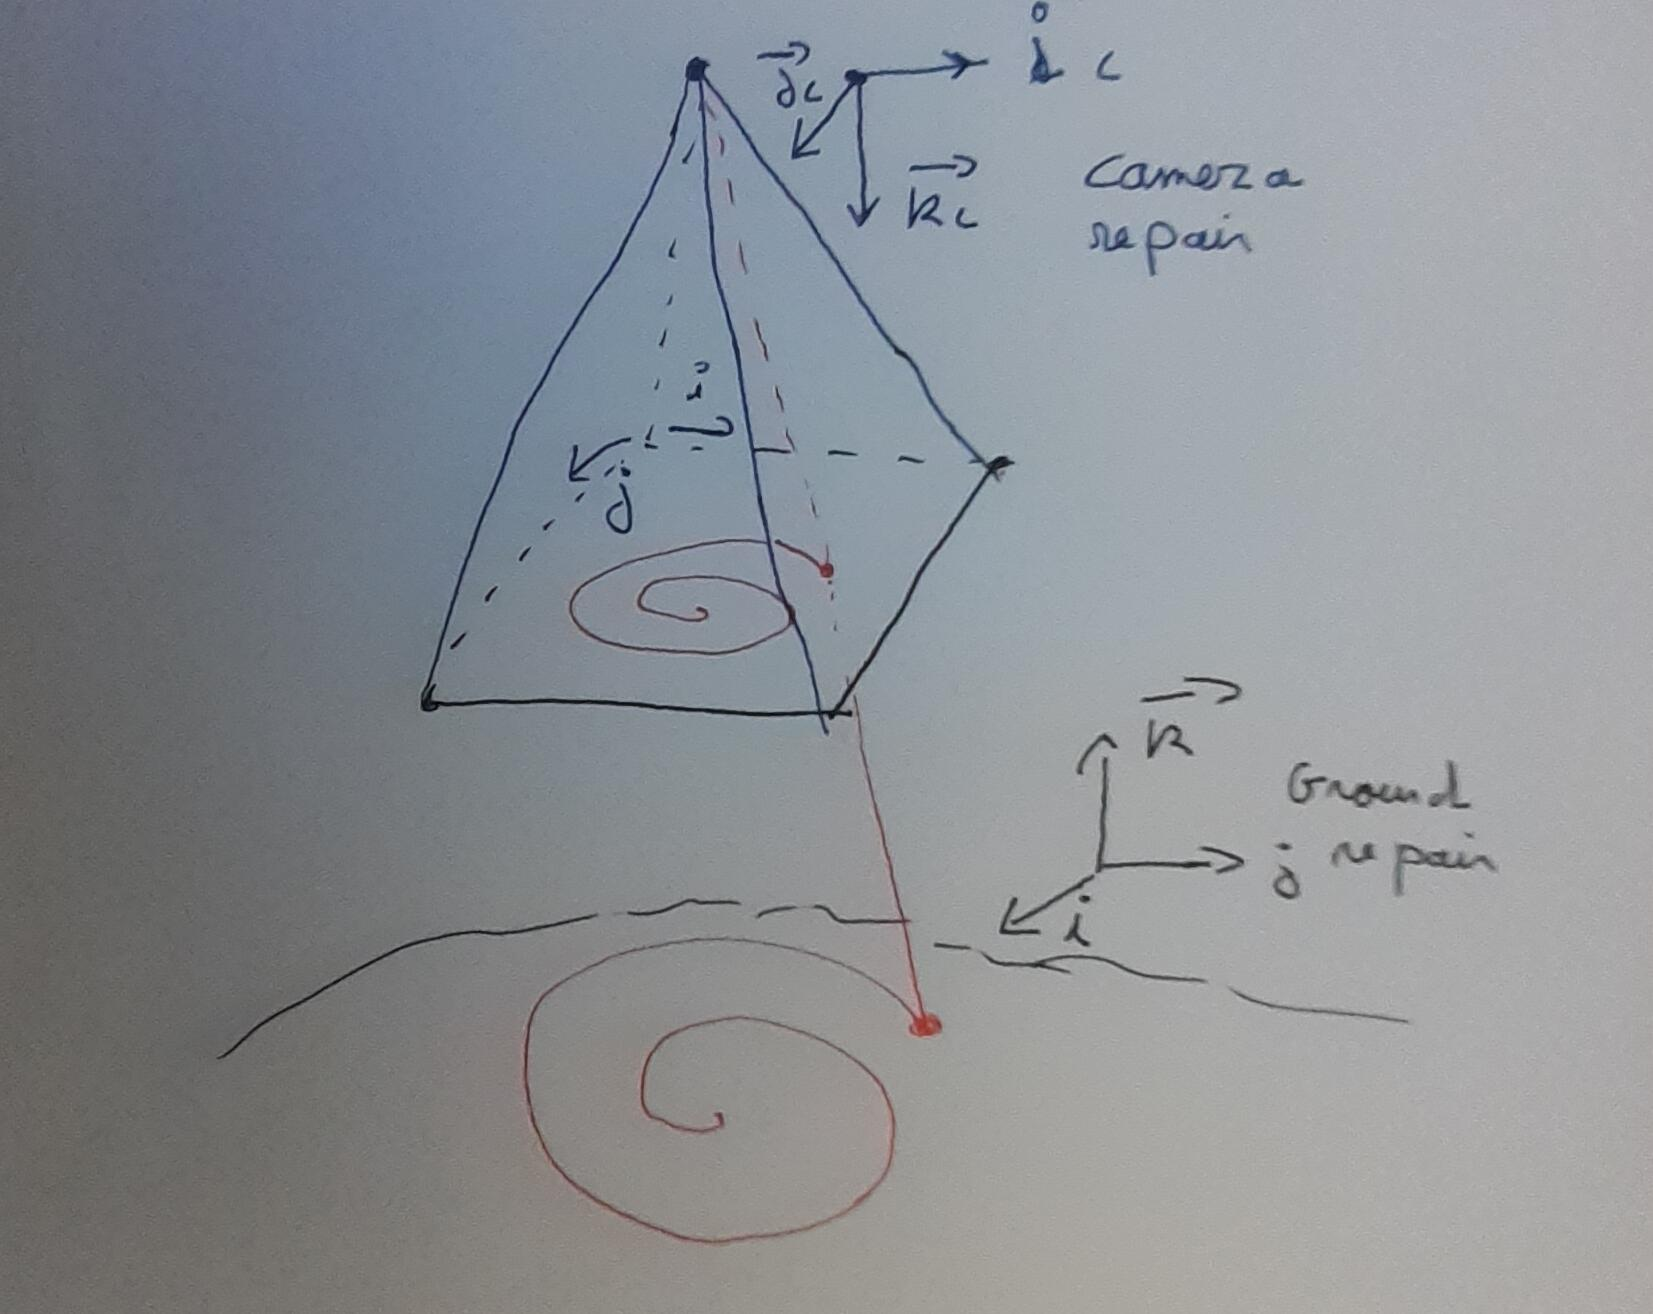
\includegraphics[width=12cm]{Methods/Images/RepairCam.jpg}
	\caption{Camera model : physically based one (left) and used one (right)}
	\label{fig:FormIm}
\end{figure}

%-----------------------------------------------------
%-----------------------------------------------------
%-----------------------------------------------------

\section{Beyond camera obscura}

%-----------------------------------------------------
\subsection{Need of lenses}

With the camera obscura, to have a sharp image we must keep a small entrance hole;
so to have enouh light we need very long exposure time. The devlopment of photography
would not have been possible without the devlopment of optic. By puting a systeme
of lenses at the entrance of the system, and being caution that the  scene focalise
on the image plane, it was possible to have a sharp image whith a sufficiently big
hole and make photography practicable.

Nowday all the camera have more or less complicated system of lenses. In fact due the
automatization of the computer added conception they tend to be more and more complex, the concepter
using the possibility offered by multiple lenses to correct more and more optical default .

For photogrammetry it change the game, because the lenses being not "infinitely thin", the gauss
condition non longer apply and some non linearity will occur , we will no longer be able to use
equation as simple as~\ref{EqIntNoDist} and will have to modelize accurately the effect of
lenses. 


%-----------------------------------------------------
\subsection{A parametric estimation issue}

A possible way to proceed would be to take into account the CAD plane of the optical
system, use in conception and to deduce the correction.  Practically, we almots never proceed
this way for two reason  :

\begin{itemize}
   \item firt this CAD plane are rarely avalaible (maybe due to industrial property ?);
   \item second, and more important, the experience prove that when we proceed to the
         modelization of two lenses from the same model, we have to modelize them with two
         different parameter if we want to get the best accuracy, so no theoreticall model 
         would fit our requirement.
\end{itemize}

So the approach currently used in photogrammetry is to select a parametric model
for the effect of lenses and to estimate the paramaters from the measures we have  (tie-point,
GCP, GNSS  \dots).


%-----------------------------------------------------
\subsection{Precaution to take}

\begin{figure}
\centering
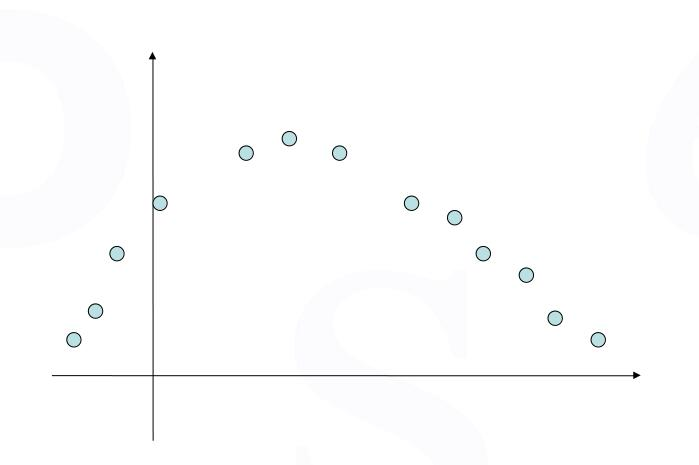
\includegraphics[width=6cm]{Methods/Images/Courbe-Pts.jpg}
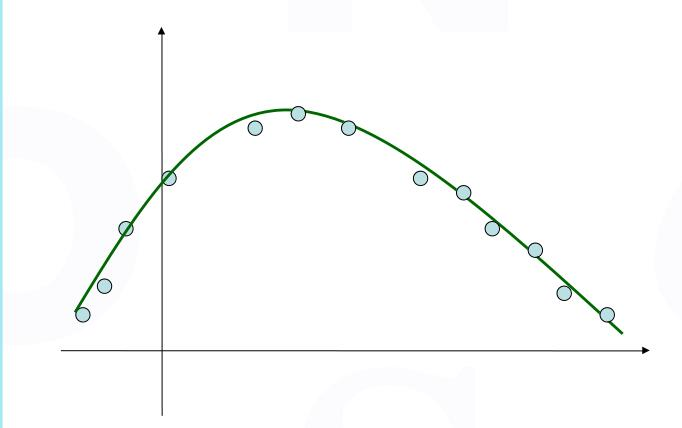
\includegraphics[width=6cm]{Methods/Images/CourbeGoodParam.jpg}\\
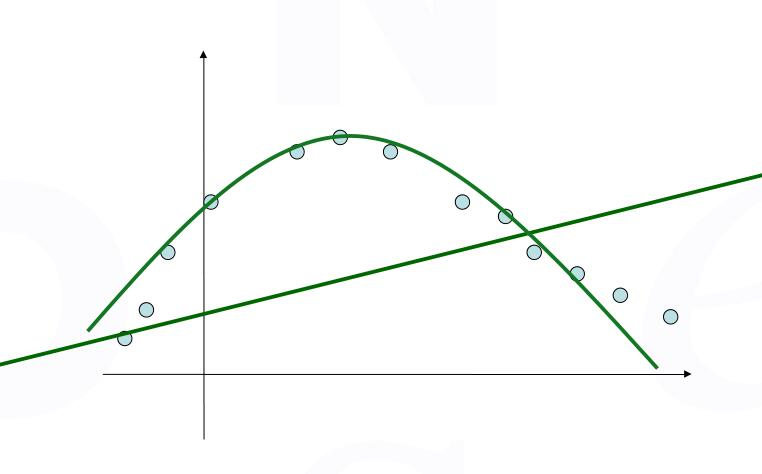
\includegraphics[width=6cm]{Methods/Images/Courbe-UndeParam.jpg}
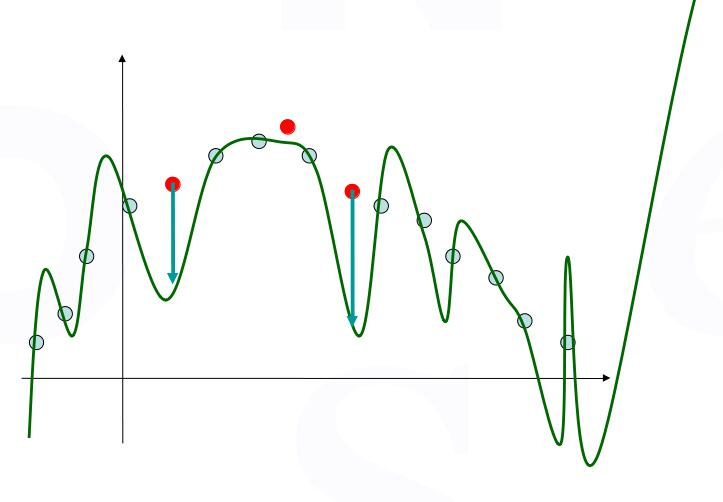
\includegraphics[width=6cm]{Methods/Images/CourbeOverParam.jpg}
	\caption{(1)Curves to interpolate (2) "Good" parametrization (3) Under parametrization (4) Over parametrization}
	\label{fig:CurvesParam}
\end{figure}


This empiricall approach does not prevent from being cautious
to the selection of model, we will have the usual compromise in the selection
of the parametric model, illustrated by figure~\ref{fig:CurvesParam}  on a problem of curve interpolation:


\begin{itemize}
	\item if we don't have enough paramater (curve 3) we are not accurate  even on the data to fit,
	   here if we fit with a straight line, or even with a parabol, we are not close to the learning data ;

   \item if we  have too many parameter (curve 4), we can have a very good match on the learning data, but have 
	 poor result as soon as we test with new data; this illustrated with  figure ??? were
         we use the "naive" lagrange interpolation to fit $N+1$ point with a $N$ degree polynomial,
         we have a perfect fit and the learning data, but a very
\end{itemize}

The question of selecting the adequate model is a difficult one, and to our best knowledge
still open in photogrammetry.  Is it preferable to have over or under paramatrization ? There
is controvorsery arguments :


\begin{itemize}
   \item  on one hand, as illustrated by figure ~\ref{fig:CurvesParam}, on can argue that under parametrization is less dangerous
         than over parametrization;

   \item  on the other hand, in "modern" photogrammetry the measurement comes more and more from automatic system,
          we can easily have several ten thousands of tie points, so one can argue that there is no real risk to have $100$ parameter
          even if we only really need $10$.
\end{itemize}

Consequently, it was thought, that the best we can do in {\tt MMVII} is to offer a sufficient large set of model
of camera, from the simple ones to the most universal one, and let the user select them according to
the precise knowledge of his domain. 

\begin{figure}
\centering
	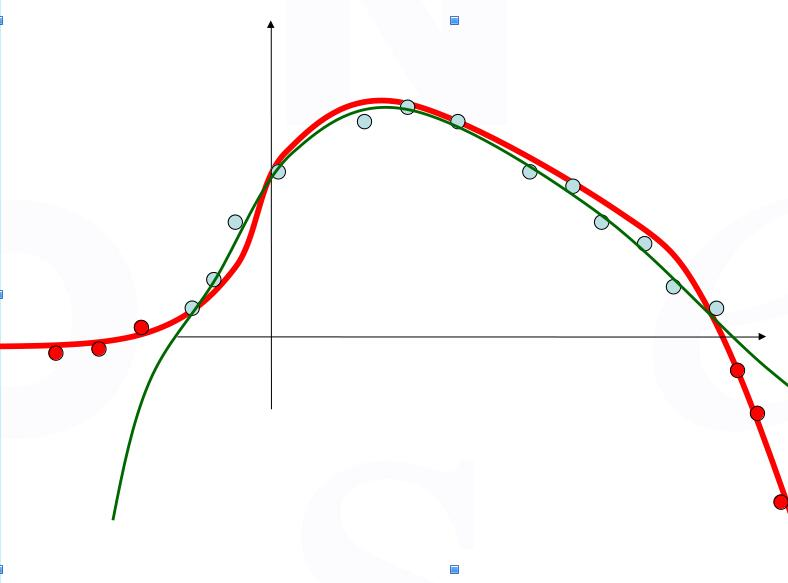
\includegraphics[width=6cm]{Methods/Images/CourbeExrapol.jpg}
	\caption{Extrapolation}
	\label{fig:CurvesExtrpol}
\end{figure}

However, even is this choice of parameter is not easy, there is
one universal rule : if can be good in interpolation, we are always bad in extrapolation
as illustrated on figure~\ref{fig:CurvesExtrpol}. A 
consequence when will estimate the model of a camera : if we have no measurement in the corners,
we are almost sure that we estimation will be poor in these corners.

%-----------------------------------------------------
\subsection{Still a central perspective, with a distorsion}
\label{Still:Persp}

In the next section we are going to introduce step by step, different model with a continuous
refinement of the physical modelization.  

\begin{figure}
\centering
	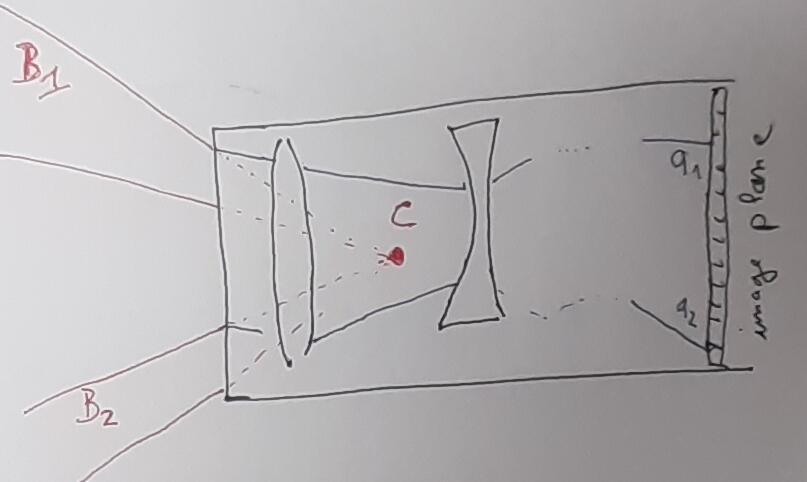
\includegraphics[width=8cm]{Methods/Images/CamPersp.jpg}
	\caption{Ligth path, all outing bundle converge to $C$}
	\label{fig:CamPerspScheme}
\end{figure}

The only hypothesis that we will maintain all allong these pages is that all the bundle issued from image
plane go through the same point $C$. This is schematised by figure~\ref{fig:CamPerspScheme} :
how complicated may be the ligth path inside the camera, we still have the property that
it exist a virtual point $C$, such that for any image point $q_i$, the bundle $B_i$ that lead to $q_i$
all go trough $C$.

This hypothesis is universally adopted, and justified because we still have a diaphragam that physicall contraint
the light to go trough it centers; of course the light will cross lenses before converning to this diaphragm but, 
, under gaussian approximation the image and reciproc image of converging bundle are still converging bundles.
To our knowledge, the only practicle cases where this hypothesis may be questionned are macro-photogrammetry and
sub-marine photogrammetry. We will discuss that ???. And maybe in the future of {\tt MMVII} project we will 
test option to relax this hypothesis for these context.

With this hypothesis, the image formation equation~\ref{FormImage0} still holds if
we add a supplentary $2d$ image deformation. Suppose in the initial simplistic camera
obscura, or even in a camera lenses satisfying gaussian approximation, 
the bundle $B_i$ would have arrived in $q^0_i$, now with the not thin lenses ,
it really arrive in $q_i$, we call $\phi$ the $2d$ mapping such that $\phi : q^0 \rightarrow q$.
With $ \mathcal{I}(q) = \phi (\mathcal{I}_0(q))  $, we have now :


\begin{equation}
	q  =   \mathcal{I} (\pi_0 (^t R (P - C)))
\end{equation}

By the way, for technicall reason we prefer to write : $ \mathcal{I}(q) = \mathcal{I}_0(D(q)) $ ; 
the reason being numericall stability of least square system, we prefer to have $D$ operate on adimentionnal numbers
(i.e as $\frac{x}{z}$).  The two modelization being obvioulsy equivalent from the pure mathematicall point of view :
as $D= \mathcal{I}_0^{-1} \circ \phi \circ  \mathcal{I}_0$.


%-----------------------------------------------------
\subsection{Summary : new image formula}

We note $D$ the additional term, classically named as distorsion. We assume for now that the gaussian approximation
globally holds,  this is the case with standard lenses, and then $D$ can be assumed to be close to identity.
This will not be the case with fish-eye, and we will see that we will proceed by replacing $\pi_0$ by other
projection.

The following three equations summarize where we are in our modelization :



\begin{equation}
	q  =   \mathcal{I} (\pi_0 (^t R (P - C))) ; \label{FormImage1}
\end{equation}

\begin{equation}
	 \mathcal{I} = \mathcal{I}_0  \circ D
\end{equation}

\begin{equation}
	  D \approx Id
\end{equation}

%-----------------------------------------------------
%-----------------------------------------------------
%-----------------------------------------------------

\section{Radial modelisation}

\subsection{Radial symetry hypothesis}

\begin{figure}
\centering
	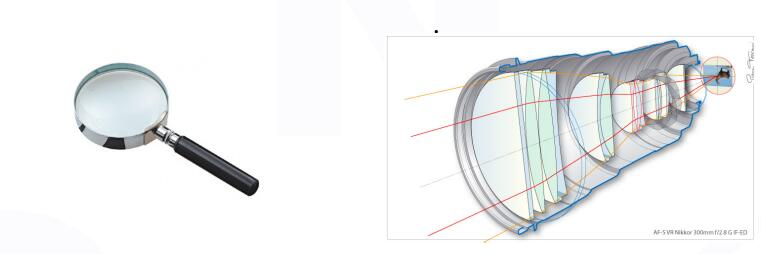
\includegraphics[width=12cm]{Methods/Images/Lenses.jpg} \\
	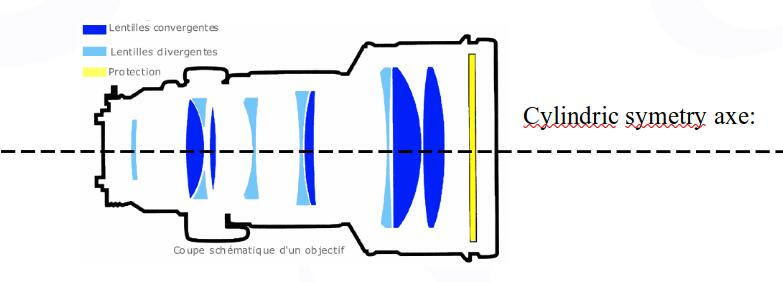
\includegraphics[width=8cm]{Methods/Images/LensesCyl.jpg}
	\caption{A single lense , and modern }
	\label{fig:Lenses}
\end{figure}

We start the modelization with two observation that are satisfied with a
high accurracy :

\begin{itemize}
    \item  each individual lense has a radial symetry arround it opticall axe;:
    \item  the mechaninal building is made so that all the lenses are aligned on
	    their common optical axe $\mathcal{A}$.
\end{itemize}


These elementary remarks have for consequence that, how sophisticated may be the combinaison
of many lenses, each having a complicated non spherical shape, we still have a global cylindrical
symetry on our system. This is illustrated by schemes of figure~\ref{fig:Lenses}.
The perspective center $C$ defined in \ref{Still:Persp}, must belong to the axes of symetry,
so we have $\mathcal{A}=(C,\vec{k})$. 


\subsection{Methodology}

\begin{figure}
\centering
	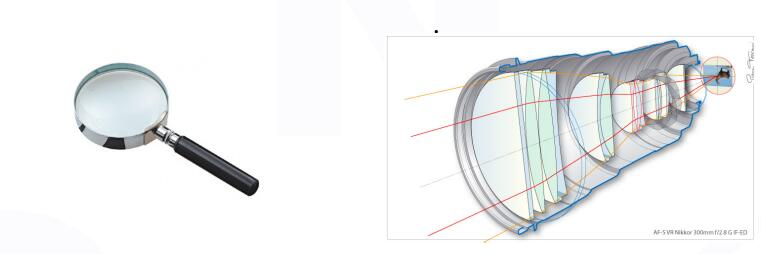
\includegraphics[width=2cm]{Methods/Images/Lenses.jpg} \\
	\label{fig:Dioptr}
\end{figure}

Let $B$ be an incoming ray, we want to establish the property of the outcoming ray $B'$
that will intersect the sensor. The optical system is made of succession of diopters $D_1,\dots D_n$,
that are have all a symetry arround $\mathcal{A}$; between to diopters $D_k$ and $D_{k+1}$, the light
is following a straight line $B_k$,  so the path going from $B$ to $B'$ can be wroten as
$B_0,B_1,\dots,B_n$ with = $B_0=B$ and $B_n=B'$ where each $B_k$ is a straigth
line segment, this is illustrated by figure~\ref{fig:Dioptr}. 

The ray $B_0$ cross $C$ and is completely caracterised by its direction $\vec{B_0}$ that
we can write in spherical coordinates :

\begin{equation}
     \vec{B_0}   =\begin{pmatrix}  \cos(\theta_0) \sin(\phi_0) \\ \sin(\theta_0) \sin(\phi_0)  \\ \cos(\phi_0) \end{pmatrix}
	     \label{PC:Spher:Coord}
\end{equation}

We want to prove the three following property :

\begin{enumerate}
    \item all $B_k$ instersect $\mathcal{A}$;
           consequently $B_k$ can be caracterised by it direction $\vec{B_k}$ and 
           the abscisse $x_k$ of its intersection with $\mathcal{A}$, we will note $\theta_k,\phi_k$
          the spherical coordinates of $\vec{B_k}$ (as in~\ref{PC:Spher:Coord});

  \item $\theta_k = \theta_0$   (i.e the path stay in the original plan containing $B_0$ and :
    \item $\phi_k = \psi_k(\theta_0)$  ;
\end{enumerate}


This is right for $B_0$ because as seen in ~\ref{Still:Persp}  all incoming ray intersect $C$
and $\mathcal{A}=(C,\vec{k})$.

We wil establish properpty between $B_k$ and $B_{k+1}$ and,
by recurence, this will establish the property for $B_n=B'$.





We note $\rho, \varphi,z$ the cylindrical coordinates :

\begin{equation}
	\begin{pmatrix} \rho \cos(\varphi)  \\ \rho\sin(\varphi)  \\ z \end{pmatrix} \label{Cyl:Coord}
\end{equation}





\subsection{Property 1}

We  want first to establish that all $B_k$ intersect the axe $\mathcal{A}$.
This is right for $B_0$ because as seen in ~\ref{Still:Persp}  all incoming ray intersect $C$
and $\mathcal{A}=(C,\vec{k})$.


Now consider a the line $B_{k-1}$ that is deflected by dioptr $D_k$ to give $B_k$, let $p_k$
be the point where $B_{k-1}$  and $B_k$ intersect $D_{k+1}$, and $\vec{n}_k$ be the normal to
to $D_k$ in $p_k$.



Let use spherical coordinate for coding  direction of bundles :



Given a set  of incoming ray  $\vec{R}(\theta,\phi)$ which all intersect point $\mathcal{A}$, we want to show that the radial symetry
implies that the outcoming $\vec{R}(\theta',\phi')$ follow the properties :

\begin{enumerate}
	\item  all the output ray belong to the axe $\mathcal{A}$ ; \label{L1}
	\item  we have $\phi' = \phi$, this means that the $3$ vector $\vec{R}(\theta,\phi)$,$\vec{k}$ and $\vec{R}(\theta',\phi')$ belong
		to the same plane; \label{L2}

	\item  
\end{enumerate}


We want to show \ref{L1} and \ref{L2}

Let $\vec{B_0}$ be a bundle entering the system, 


We have a succession of bundles that cross interface different interface $\vec{B_k} = \vec{R}(\theta_k,\phi_k)$.
Let show first that $\phi_0 = \phi_1 \dots = \phi_n$.
$B_0$ cross the interface in

due to the symetry of the system,





%-----------------------------------------------------
%-----------------------------------------------------
%-----------------------------------------------------

\section{Decentric distorsion}


%-----------------------------------------------------
%-----------------------------------------------------
%-----------------------------------------------------

\section{General model}

\subsection{Fish eye model}
\subsection{$360$ camera}
\subsection{Assemblage camera}

%-----------------------------------------------------
%-----------------------------------------------------
%-----------------------------------------------------

\section{Planary inclinaison}




